\documentclass[final]{beamer}
\mode<presentation>
  {
   \usetheme{GP}
  }
\usepackage{times}
\usepackage{amsmath,amsthm, amssymb, latexsym}
%\boldmath
\usepackage[english]{babel}
\usepackage[utf8]{inputenc}
\usepackage{ragged2e} 
\usepackage[orientation=landscape,size=a0,scale=1.1]{beamerposter}
\usepackage{color}
\usepackage{framed,color}
\graphicspath{{figs/},{GenExamples/}} % modify XXX

% For algorithms
\usepackage{algorithm}
%\usepackage[]{algorithm2e}
\usepackage{algorithmic}
\newlength\myindent
\setlength\myindent{5em}
\newcommand\bindent{%
  \begingroup
  \setlength{\itemindent}{\myindent}
  \addtolength{\algorithmicindent}{\myindent}
}
\newcommand\eindent{\endgroup}


\usepackage{graphicx}
\usepackage{subfigure}
%\usepackage[orientation=portrait,size=a0,scale=1.0]{beamerposter}

%\graphicspath{{figures/}}


\setlength{\leftmargini}{4em}


\renewcommand{\vec}[1]{{\mathbf{#1}}}
\definecolor{amber}{rgb}{1.0, 0.75, 0.0}
\definecolor{bananayellow}{rgb}{1.0, 0.88, 0.21}
\definecolor{ballblue}{rgb}{0.13, 0.67, 0.8}
\definecolor{brass}{rgb}{0.71, 0.65, 0.26}
\definecolor{byzantine}{rgb}{0.74, 0.2, 0.64}

%\definecolor{dg}{rgb}{0.45, 0.76, 0.46}
\definecolor{dg}{rgb}{0.00, 0.55, 0.00}

\newcommand{\ytheta}{\normalsize$\mathcal{L}(\theta)$}
%\newcommand{\highlight}[1]{\textcolor{lblue}{\textbf{#1}}}
\newcommand{\highlight}[1]{\textcolor{blocktbgn}{#1}}

\newcommand{\headline}[1]{\vspace{1cm}\begin{center}\textbf{#1}\end{center}\vspace{0.5cm}}
\newcommand{\subhead}[1]{ \centering \textbf{#1}                                                                                                                                                                 \vskip-1.7\baselineskip~\\
\rule{\linewidth}{1pt}
\vspace{-0.9cm}
}


\newcommand{\smallblock}[2]{
  \vskip0.1cm
  \begin{beamercolorbox}[leftskip=1cm,colsep*=.75ex,rounded=true,shadow=true]{block title}%
    \usebeamerfont*{block title}\small #1
  \end{beamercolorbox}%
  {\ifbeamercolorempty[bg]{block body}{}{\nointerlineskip\vskip-0.5pt}}%
  \usebeamerfont{block body}%
  \begin{beamercolorbox}[colsep*=.75ex,sep=.75ex,vmode,rounded=true,shadow=true]{block body}%
  #2
  \end{beamercolorbox}
}

%%%%%%%%%%%%%%%%%%%%%%%%%%%%%%%%%%%%%%%%%5
% Custom Commands


% ---------- commands ----------
\newcommand{\x}{\ensuremath{\times}}
\newcommand{\disT}{\textstyle}
\newcommand{\disS}{\displaystyle}
\newcommand{\prob}[2]{p(#1 \, | \, #2)}  % nicely space p(1 | 2)
\newcommand{\Prime}{\,'}  % nicely space p(1 | 2)
\newcommand{\One}{I}
\renewcommand{\vec}[1]{{\mathbf{#1}}}
\newcommand{\Kn}{\mathcal{K}_{n}}
\newcommand{\Ih}{\mathcal{I}_{n}}
\newcommand{\Sh}{\mathcal{S}_{h}}
\newcommand{\Ss}{\mathcal{S}}
%-----------------------------------

\newcommand{\Bernoulli}{\mathcal{B}}

\newcommand{\sVec}{\vec{s}}
\newcommand{\sVecN}{\vec{s}^{\,(n)}}
\newcommand{\yVec}{\vec{y}}
\newcommand{\yVecN}{\vec{y}^{\,(n)}}
\newcommand{\yN}{y^{(n)}}





\newcommand{\E}[1]{\left\langle{}#1\right\rangle}



\newcommand{\Ncal}{{\cal N}}
\newcommand{\sigSq}{\sigma^2}
\def\One{\hbox{$1\hskip -1.2pt\vrule depth 0pt height 1.6ex width 0.7pt\vrule depth 0pt height 0.3pt width 0.12em$}}


\newcommand{\RRR}{\mathbb{R}}


\newcommand{\fix}{\marginpar{FIX}}
\newcommand{\new}{\marginpar{NEW}}



\newcommand{\sVecPrime}{\vec{s}^{\,\prime}}


\newcommand{\LL}{\mathcal{L}}

%
\newcommand{\tr}{\ensuremath{^\mathsf{T}}}
%

\newcommand{\YCal}{{\cal Y}}
%
\newcommand{\Old}{\mathrm{old}}
%
\newcommand{\Wid}{W_{id}}
\newcommand{\WidPrime}{W_{id^{\prime}}}
\newcommand{\WidPrimeOld}{W_{id^{\prime}}^{\mathrm{old}}}
\newcommand{\WidOld}{W_{id}^{\mathrm{old}}}
\newcommand{\Whd}{W_{hd}}
\newcommand{\WTilde}{\tilde{W}}
\newcommand{\WEff}{W^{\mathrm{eff}}}
\newcommand{\WOld}{W^{\prime}}
%\newcommand{\WOld}{W^{\mathrm{o}}}
%\newcommand{\WOld}{W^{\mathrm{old}}}
\newcommand{\Wg}{W^{\mathrm{gen}}}
\newcommand{\WTildeOld}{\tilde{W}^{\mathrm{old}}}
%
%\renewcommand{\Wt}{{\cal W}}
%
%\newcommand{\Wnn}{\tilde{W}}
\newcommand{\Wnn}{{\cal W}}
\newcommand{\Wnnid}{\Wnn_{id}}
\newcommand{\WnnidPrime}{\Wnn_{id^{\prime}}}
\newcommand{\WnnidPrimeOld}{\Wnn_{id^{\prime}}^{\prime}}
\newcommand{\WnnidOld}{\Wnn_{id}^{\prime}}
\newcommand{\WnnidNew}{\Wnn_{id}^{\mathrm{new}}}
\newcommand{\Wnnhd}{\Wnn_{hd}}
\newcommand{\WnnTilde}{\tilde{\Wnn}}
\newcommand{\WnnEff}{\Wnn^{\mathrm{eff}}}
\newcommand{\WnnBar}{\overline{\Wnn}}
\newcommand{\WnnOld}{\Wnn^{\mathrm{old}}}
\newcommand{\WnnTildeOld}{\tilde{\Wnn}^{\mathrm{old}}}
\newcommand{\WDiffThres}{\theta_{\Delta{}W}}
\newcommand{\Wub}{W^{\mathrm{ub}}}
\newcommand{\WVecub}{\vec{W}^{\mathrm{ub}}}
%
\newcommand{\II}{{\cal I}}
%
\newcommand{\dPrime}{d^\prime}
%
%\newcommand{\qSVecNYVecNThetaOld}{q(\sVecN; \ThetaOld)}
\newcommand{\qSVecNYVecNThetaOld}{q(\sVecN\,|\,\ThetaOld)}
%
\newcommand{\maxH}[1]{\max_{h=1,\ldots,H}\{#1\}}%
\newcommand{\limRho}{\lim_{\rho\rightarrow\infty}}
\newcommand{\prodCond}[2]{\prod_{\mbox{\scriptsize{}$\begin{array}{c}#1\\#2\end{array}$}}}
\newcommand{\sumCond}[2]{\sum_{\mbox{\scriptsize{}$\begin{array}{c}#1\\#2\end{array}$}}}
\newcommand{\vPhantom}{\phantom{\mbox{$\disS\int_a^a$}}}%
\newcommand{\vPhantomBig}{\phantom{\mbox{$\disS\int_f^f$}}}%
%
%\newcommand{\HHTwo}{\HH_{\frac{1}{2}}}
\newcommand{\HHTwo}{\HH}
%
%
\newcommand{\IN}{I^{(n)}}
\newcommand{\ItN}{\tilde{I}^{(n)}}
\newcommand{\Imax}{\mbox{$I^\mathrm{max}$}}
%
\newcommand{\piVec}{\vec{\pi}}
%\newcommand{\piVecOld}{\vec{\pi}^{\mathrm{old}}}
\newcommand{\piVecOld}{\vec{\pi}^{\prime}}
\newcommand{\piBar}{\overline{\pi}}
\newcommand{\piBarVec}{\overline{\piVec}}
\newcommand{\piVecBar}{\overline{\piVec}}
\newcommand{\piVecG}{\piVec^\mathrm{gen}}
\newcommand{\piG}{\pi^\mathrm{gen}}
%
\newcommand{\gPrime}{g^{\prime}}
\newcommand{\gammaPrime}{\gamma^{\,\prime}}
%
\newcommand{\argmax}{\mathrm{argmax}}
%
\newcommand{\hPrime}{{h^{\prime}}}


\newcommand{\OO}{\mbox{{\cal OO}}}
\newcommand{\ZZ}{{\cal Z}}

\newcommand{\ZZZplus}{\mathbb{Z}_{+}}

%
\newcommand{\KK}{{\cal K}}
\newcommand{\KKn}{\KK_{n}}
\newcommand{\HPrime}{H^{\prime}}
\newcommand{\Hprime}{H^{\prime}}
%
\newcommand{\Nt}{\mbox{$\tilde{N}$}}
\newcommand{\NNgz}{N^{^{>0}}}
\newcommand{\NSmall}{{\cal N}^{^{\leq{}2}}}
\newcommand{\NtSmall}{\tilde{{\cal N}}^{^{\leq{}2}}}
\newcommand{\Ncut}{N^{\mathrm{cut}}}
\newcommand{\NsVecKK}{N(\KK)}
\newcommand{\NsVecKKn}{N(\KKn)}


\newcommand{\disAlt}{}
%\newcommand{\disAlt}{\disT}

\definecolor{Red}{rgb}{1.0,0,0} 

\newcommand{\comment}[1]{}
%\newcommand{\comment}[1]{\textcolor{Red}{[#1]}}

\newcommand{\DKL}{D_{KL}}

\newcommand{\WGen}{W^{\mathrm{gen}}}


\newcommand{\FFt}{\tilde{\FF}}

%\newcommand{\ThetaOld}{\Theta^{\prime}}
%\newcommand{\ThetaOld}{\Theta^{\mathrm{o}}}
\newcommand{\ThetaOld}{\Theta^{\mathrm{old}}}
\newcommand{\ThetaTilde}{\tilde{\Theta}}
\newcommand{\ThetaTildeOld}{\ThetaTilde^{\mathrm{old}}}

%\newcommand{\qn}{q^{(n)}}
\newcommand{\qn}{q_n}
%\newcommand{\qnPrime}{q^{(n^\prime)}}
\newcommand{\qnPrime}{q_{n^\prime}}
\newcommand{\qt}{\tilde{q}}
\newcommand{\qnt}{\tilde{q}^{(n)}}
%\newcommand{\qnbar}{\overline{q}^{(n)}}
\newcommand{\qnbar}{\qn}
\newcommand{\dagg}{^{\dagger}}
\newcommand{\daggOne}{^{\dagger{}1}}
\newcommand{\daggZero}{^{\dagger{}0}}
\newcommand{\astt}{^{\ast}}
\newcommand{\NGauss}{{\cal N}}

%\newcommand{\One}{\dblone}
\newcommand{\Scal}{{\cal S}}
\newcommand{\BigO}{\mathcal{O}}
\newcommand{\xbf}{\mathbf{x}}

%%% MESS ABOVE %%%

\definecolor{mygreen}{rgb}{0.45, 0.76, 0.46}
\definecolor{myblue}{rgb}{0.26, 0.55, 0.76}

\fboxrule3.0mm
\fboxsep5.0mm

%%%%%%%%%%%%%%%%%%%%%%%%%%%%%%%%%%%%%%%%%%%%%%%%%%%%%%%%%%%%%%%%%%%%%%%%%%%%%%%%%
\title[]{\huge GP-select: Accelerating EM using adaptive subspace preselection}
\author[Shelton, Gasthaus, Dai, L\"{u}cke, \& Gretton]{\Large Jacquelyn A. Shelton$^{ 1}$,  Jan Gasthaus$^{ 2,3}$, Zhenwen Dai$^{ 4}$, J\"org L\"{u}cke$^{ 5}$, and  Arthur Gretton$^{ 2}$}
%\author[Shelton, \& Lampert]{Jacquelyn A. Shelton$^{1}$ and Christoph H. Lampert$^{2}$}
\institute[TU]{\large $^{ 1}$Technical University Berlin,\quad 
$^{ 2}$UCL Gatsby and CSML,\quad 
$^{ 3}$Amazon,\quad 
$^{ 4}$University of Sheffield,\quad 
$^{ 5}$University of Oldenburg}
%                $^{2}$Institute of Science and Technology Austria (IST Austria)}% \quad $^{2}$Volen Center for Complex Systems. Brandeis University, USA}
%%%%%%%%%%%%%%%%%%%%%%%%%%%%%%%%%%%%%%%%%%%%%%%%%%%%%%%%%%%%%%%%%%%%%%%%%%%%%%%%%
%  1st collumn
%%%%%%%%%%%%%%%%%%%%%%%%%%%%%%%%%%%%%%%%%%%%%%%%%%%%%%%%%%%%%%%%%%%%%%%%%%%%%%%%%%%

\begin{document}
\begin{frame}{} 
  \begin{columns}[t]
  \begin{column}{.33\linewidth}

    % ---- highlights ----
    \begin{block}{Highlights/Abstract}%{Introduction} %Abstract?  Intro & Conclusions?
            \vspace{-.4cm}  
            \begin{itemize}
            \setlength{\labelsep}{0.5em}
            \item Novel nonparametric procedure for \highlight{fast inference} in \highlight{generative graphical models with large $\#$ of latent states}, e.g. $\# latent$ $states^{\# latent}$$^{variables}$ %exponential in the number of latent variables
            \item \highlight{Idea}: meta-algorithm for EM, \highlight{iterative latent variable preselection} -- alternate between learning a \highlight{'selection function'} (reveal the relevant latent variables) and using the result for a \highlight{compact approx of the posterior distribution for EM}
          %  \item Enables inference with many latent states where exact approaches are computationally infeasible.
            \item \highlight{How}: \textcolor{dg}{learn selection function} entirely from the observed data and current EM state via \highlight{Gaussian process regression} -- earlier approaches used \textcolor{red}{expensive manually-designed selection functions} for each problem setting -- our approach is \textcolor{dg}{fully automatic and flexible}
      %%      \item \highlight{Idea}: Use GPs to approximate complex/intractable probabilistic models
            \item \highlight{Experiments} suggest GP-select to play a \textcolor{dg}{crucial role} for inference in complex hierarchical models (e.g. [1]) where the \textcolor{dg}{relationship between inputs / outputs is complex} and thus hand-derived selection functions are expensive (or impossible) %-- demonstrated here in the heirarchical model of [1]
            \end{itemize}


    % ---- setting -----
     %   \vspace{.5cm}
      %    \textbf{Problem setting:}%{Method: Adaptive Gibbs sampling in factor graphs}
       %   \vspace{-.2cm}
        %   \begin{itemize}
         %   \setlength{\labelsep}{0.5em}
          %  \item Use GPs to approximate complex/intractable probabilistic models
           % \item Selection of latent variables by learning a nonparametric relevance function, for use in ET. 
           %\end{itemize}

    \vspace{-.3cm}
    \end{block}

    % ---- bound ----
    \begin{block}{Variable selection for accelerated inference}
          \vspace{-.5cm}

        \textbf{Notation:} \\
% TODO condense!~!  i.e. y^(n) = ... for all n = 1...N
%
\begin{itemize}
\item \highlight{Observed data}: $\vec{y}^{(n)} = ( y_1^{(n)}, \dots, y_D^{(n)})^\mathrm{T}$, $N$ observations of $D$ dimensions

%%%$\vec{Y}=(\vec{y}^{(1)}, \dots, \vec{y}^{(N)})$; each vector $\vec{y}^{(n)} = ( y_1^{(n)}, \dots, y_D^{(n)})^\mathrm{T}$ is $n$th obs in a $D$-dim space ($D\times N$ matrix)\\

\item \highlight{Binary latent variables}: $\vec{s}^{(n)}=(s_1^{(n)}\dots, s^{(n)}_H)^\mathrm{T} \in \{0,1\}^{H}$, $H$ latent dims
%\footnote{We restrict ourselves to binary latent variables here, though discrete variables with higher cardinality can easily be used by converting them into binary variables.} 
%%% $\vec{S} = (\vec{s}^{(1)}, \dots, \vec{s}^{(N)})\in \{0,1\}^{H \times N}$; each $\vec{s}^{(n)}=(s_1^{(n)}\dots, s^{(n)}_H)^\mathrm{T} \in \{0,1\}^{H}$ is $n$th vector in $H$-dime latent space, and each individual hidden variable $h=1,\dots,H$, the vector $\vec{s}_h=(s_h^{(1)}\dots, s^{(N)}_h)\in \{0,1\}^{N}$. \\
\item \highlight{Reduced latent space}: $H\,'$-dimensional, where $H\,' \ll H$ dimensions.
%Note that although we restrict ourselves to binary latent variables here, discrete variables with higher cardinality can easily be used by converting them into binary variables.

\item \highlight{Prior distribution over latent variables} is $p(\vec{s} | \theta)$, \highlight{likelihood of the data} is $p(\vec{y} | \vec{s}, \theta)$ $\rightarrow$ \highlight{Posterior distribution over latent variables}: 
%
\vspace{-.05cm}
\normalsize
\begin{equation}
\label{eq:post}
p(\vec{s}^{(n)}|\vec{y}^{(n)},\Theta)  = \frac{p(\vec{s} | \Theta) \, p(\vec{y} | \vec{s}, \Theta)}
{\disS\hspace{-1.5mm}\sum_{\vec{s}\Prime^{(n)}} p(\vec{s}\Prime | \Theta) \, p(\vec{y} | \vec{s}\Prime, \Theta)}
\end{equation}
\large

\end{itemize}

        \subhead{Selection via Expectation Truncation (ET) [2] in EM}
           \begin{itemize}
            \setlength{\labelsep}{0.5em}
            \item \highlight{Posterior distribution~\eqref{eq:post}} approximated by a truncated posterior distribution, computed with \highlight{support reduced to $\Kn$}:
                %
                \vspace{-.1cm}
                \normalsize
                \begin{align}
                \label{eq:sel-post}
                p(&\vec{s}^{(n)}|\vec{y}^{(n)},\Theta) 
                &\approx q_n(\vec{s}^{(n)};\Theta) = \frac{p(\vec{s}^{(n)},\vec{y}^{(n)}|\,\Theta) \,\delta(\vec{s}^{(n)}\in\,\,\Kn)}
                   %{\ disS\hspace{-1.5mm}\int_{\vec{s}\Prime^{(n)}\in\mathcal{K}_n}\hspace{-8mm} p(\vec{s}\Prime^{(n)},\vec{y}^{(n)}|\,\Theta)\,d\vec{s}\Prime^{(n)}}
                {\disS\hspace{-1.5mm}\sum_{\vec{s}\Prime^{(n)}\in\mathcal{K}_n}\hspace{-3mm} p(\vec{s}\Prime^{(n)},\vec{y}^{(n)}|\,\Theta)}
                \end{align}
                %
                \large
                \highlight{-} where $\Kn$ contains the latent states of the $H'$ relevant variables for data \\
                $\:\:$ point $\vec{y}^{(n)}$, and $\delta(\vec{s}\in\mathcal{K}_n)=1$ if
                $\vec{s}\in\mathcal{K}_n$, else $0$, \\
                \highlight{- $\Kn$} should contain \highlight{most of the probability mass} $\prob{\vec{s}}{\vec{y}}$, and\\
                \highlight{- $\Kn$} should be significantly \highlight{smaller than full latent space}
           \end{itemize}

         
        \subhead{ET with affinity}
          \vspace{-.2cm}
           \begin{itemize}
            \setlength{\labelsep}{0.5em}

            \item \highlight{Constructing a selection function} %$\mathcal{S}^{(n)}$ 
first, rank the latent variables according to an 
\highlight{\emph{affinity function}} $f_h(\vec{y}^{(n)}) : \mathrm{R}^D \mapsto \mathrm{R}$ %^{+}$
which directly reflects the \highlight{relevance of latent variable $s_h$}. 

            \item A natural choice of \highlight{selection function} is the one that \highlight{\emph{approximates the marginal posterior probability}}
                of each variable, e.g.\ learn \highlight{$f$} as follows:
                %
                \begin{equation}
                \label{eq:affinity}
                f_h(\vec{y}^{(n)}) %= \hat{{p}}^{(n)} 
                    \approx p^{(n)}_h \equiv p(s^{(n)}_h = 1|\vec{y}^{(n)}, \Theta)
                \end{equation}
                %

        \highlight{$\rightarrow$} Use the affinity function to \highlight{select relevant variables}: marginal posterior probability \highlight{$p_h$ exceeds a threshold}
         \end{itemize}
    \vspace{-.7cm}
    \end{block}

  \end{column}
  %%%%%%%%%%%%%%%%%%%%%%%%%%%%%%%%%%%%%%%%%%%%%%%%%%%%%%%%%%%%%%%%%%%%%%%%%%%%%%
  % 2nd column
  %%%%%%%%%%%%%%%%%%%%%%%%%%%%%%%%%%%%%%%%%%%%%%%%%%%%%%%%%%%%%%%%%%%%%%%%%%%%%%
  \begin{column}{.35\linewidth}

    \begin{block}{Latent Variable Preselection: affinity and GP-Select}
          \vspace{-.4cm}
            \begin{center} 
 
            \vspace{.1cm}
            \includegraphics[width=.42\textwidth]{graph-affinity2.pdf}\\
           \textcolor{blocktbgn}{Affinity (approx marg post prob) to highlight most relevant latent variables}
            \end{center}
       
        
         \vspace{-.05cm}
           \begin{itemize}
            \setlength{\labelsep}{0.5em}

            %%%\item $f_h$ to approximate the marginal posterior probability $p_h$ that $s_h^{(n)}=1$.
            \item \highlight{Sort and reduce} full indices to $H\,'$ most rel. variables' set -- define 
                  \highlight{$\gamma\,(\hat{\vec{p}}^{(n)})$} to output the \highlight{$H\,'$ selected variable indices $I$} for the $n$th data point
                  %From $\hat{p}_{h=1}^{(n)},\dots, \hat{p}_H^{(n)}$, 
            \item \highlight{Define subset} of the $H\,'$-dimensional \highlight{relevant latent states $\Kn$} with \highlight{$\mathcal{I}(I)$} 
                %for the $n$th data point
                %Finally, using the indices $I$ from $\gamma$, we define $\mathcal{I}(I)$ to return an 
                %$H'$-dimensional subset of selected relevant latent states $\Kn$ for each data point $\vec{y}^{(n)}$. 
            \item All \highlight{non-relevant variable states} $s_h$ for all variables $h\not\in I$ are \highlight{set to $0$} in Eq.~\eqref{eq:sel-post} 
 %are effectively set to $0$ in Equation~\eqref{eq:sel-post} by not being present in the state set $\Kn$.
            \item Using $\vec{f}$, $\mathcal{I}$, and $\gamma$, we can define a 
            \highlight{\emph{selection function}} $\mathcal{S}: \mathrm{R}^D \mapsto 2^{ \{1,\dots,H \}}$ 
            to \highlight{select subsets $\mathcal{K}_n$} per data point $\vec{y}^{(n)}$ for
            the \highlight{affinity based selection function}:
            %
            \vspace{.2cm}
            \begin{equation}\label{eq:sel-func}
            \mathcal{S}(\vec{y}^{(n)}) \;=\; \mathcal{I} \left[  \gamma \left[ \vec{f}(\vec{y}^{(n)}) \right]  \right] \;=\; \mathcal{K}_n
            \end{equation}
        \end{itemize}

      \vspace{.35cm}
      \subhead{GP-select: Learn affinity with GP regression}    
        \vspace{-.2cm}
           \begin{itemize}
            \setlength{\labelsep}{0.5em}

            \item \highlight{Previous work}: \highlight{selection function} $\mathcal{S}$ was \highlight{deterministic and derived by hand} for each model using upper bounds or noiseless limits [3,4]
%hand-crafted to model the properties of the graphical model of interest, using intuition from noiseless limits or upper-bound results specific to the model 
%\citep{LuckeEggert2010,SheltonEtAl2012,BornscheinEtAl2013,SheikhEtAl2014}.

            \item We \highlight{generalize and automatize} this approach:  %for inference in graphical models
%instead of a predefined form of $\Ss$ for variable selection, learn it in black-box and model-free way based on the data.
                \highlight{learn $Ss$} with \highlight{GP regression} %-- flexible and can make exact predictions
            \item Define $f_h(\vec{y}^{(n)}) \sim \text{GP}\left(0, \, k(\cdot,\cdot) \right)$, where $k(\cdot, \cdot)$ is the covariance kernel and flexibly parameterizable to represent the relationship between variables
%flexibly govern the representation of the relationship between variables.
%%%Again, we use $f_h$ to approximate the marginal posterior probability $p_h$ that $s_h^{(n)}=1$.

            \item Before each E-step: 
%%%compute selection function $\mathcal{S}$ by calculating affinity using a GP to regress the expected values of the latent variables $\langle \vec{S} \rangle$ onto the observed data $\vec{Y}$ -- 
                \highlight{train GP on $p_h$ from prev. EM iteration} (where $p_h = \langle s_h \rangle$): 
            $\mathcal{D} = \{ (\vec{y}^{(n)}, \langle\vec{s}\rangle^{(n)}_{q_n(\vec{s})}) | n = 1,\dots, N \}$

            \item \highlight{Compute} predicted mean of GP using \highlight{leave-one-out (LOO) prediction}:

                \vspace{-.6cm}  % (*1)
                \begin{equation}\label{eq:gp-loo}
                %\vec{\mu}^{(n)} \;=\;  \hat{\vec{s}}^{(n)} \;=\;  
                %\hat{p}_{h}^{(n)} =   
                %p_{h}^{(n)} - \frac{ [ K^{-1} \vec{p}_{h} ]_{nn} }{ [ K^{-1} ]_{nn} }.
                \hat{p}_{h}^{(n)} \leftarrow   
                \langle s \rangle_h^{(n)} - \frac{ [ K^{-1} \langle\vec{s}\rangle_{h} ]_{nn} }{ [ K^{-1} ]_{nn} }
                \end{equation}
                %
                \vspace{.4cm}
                \highlight{$\rightarrow$ Efficiently implementable} for all latent vars $h=1,...,H$ and data points $n=1,...,N$ using matrix operations -- only $1$ kernel matrix inversion for all $N$
            \item \highlight{Substitute} Eq.~\eqref{eq:gp-loo} for $\vec{f}$ in the affinity based selection function Eq.~\eqref{eq:sel-func} %$\Rightarrow$ GP-select

           \end{itemize}
    \end{block}


  \begin{block}{Algorithm}%: GP-Select to accelerate inference in EM}
    \vspace{-1cm}
    \begin{algorithm}[H] 
    %%\caption{GP-Select to accelerate inference in Expectation Maximization}
    \label{alg:gp-select}
    \begin{algorithmic}
    \FOR{EM iterations $t=1,\dots,T$}\STATE{\vspace{-1cm}    
        \bindent        
        \FOR{data point $n=1,\dots, N$}
        %\bindent
        \STATE{
            $\qquad$ compute affinity of all latent variables $\hat{\vec{p}}_t^{(n)}$: \eqref{eq:gp-loo}\\
        %2. sort and reduce indices to $H'$\\
         %   2.2. include uniformly chosen indices\\
           $\qquad$  compute subset of relevant states $\Ss$: \eqref{eq:sel-func}\\ % get $\Kn$ 
        %3. puke out reduced set of latent states $\Kn$ to use to calculate posterior distribution in E-step\\
           $\qquad$ compute truncated posterior $q_{n,t}(\vec{s})$, E-step: \eqref{eq:sel-post}\\ % on reduced set $\Kn$
           $\qquad$ update model parameters in M-step\\ 
           $\qquad$ store $\langle \vec{s} \rangle^{(n)}_{q_{t}(\vec{s})}$ for $\vec{p}^{(n)}$ in EM iteration ${t+1}$\\
        }%\eindent
        \ENDFOR\\%\vspace{-.2cm}
        
        $\qquad$optimize kernel hyperparams every $T^{*}$ EM iterations
        \eindent
    }%\vspace{-.2cm}
    \ENDFOR
    \end{algorithmic}
    \end{algorithm}
    \vspace{-1.3cm}

    \end{block}



  \end{column}


  %%%%%%%%%%%%%%%%%%%%%%%%%%%%%%%%%%%%%%%%%%%%%%%%%%%%%%%%%%%%%%%%%%%%%%%%%%%%%%
  % 3nd column
  %%%%%%%%%%%%%%%%%%%%%%%%%%%%%%%%%%%%%%%%%%%%%%%%%%%%%%%%%%%%%%%%%%%%%%%%%%%%%%
  \begin{column}{.32\linewidth}
    \begin{block}{Experiments}
      %\large

    \vspace{-.5cm}
      \subhead{Sparse coding models}
    %   \textcolor{blocktbgn}{Data \& dictionary elemements} 
            \vspace{.25cm}
                \includegraphics[width=.81\textwidth]{sparsecoding/bars-test_transpose.pdf}\\
                %
            \vspace{.05cm}
           \begin{itemize}
            \item \highlight{Data}: $N=2,000$ with $D=5\times5$ obs dims \& \highlight{$H=10$ latent dims/bars} gen. by each model, with
                \highlight{GP-select} to preselect \highlight{$H\,' = 5$ dims}
            \item \highlight{Shown}: final EM it; GP-select \highlight{converges to GT params}, $W_{GP-select}$ % as w. hand-crafted sel functions ($W_{hand-craft}$) .
                    % Observed empirically: composition kernel flexibly subsumes other kernels,suggesting it a good choice for general use.
          \end{itemize}

\vspace{.2cm}
     \subhead{Gaussian mixture model} 
        %\textcolor{blocktbgn}{Gaussian mixture model} 
%\vspace{-.1cm}
        \vspace{.15cm}
        %    \begin{center}
                \includegraphics[width=.79\textwidth]{mog/mog_labels2.pdf}\\
         %   \end{center}
            %
           \vspace{.2cm}
           \begin{itemize}
            \item \highlight{Data}: \highlight{$C=3$ clusters}, \highlight{GP-select} to preselect \highlight{$C\,'=2$ clusters}
            \item \highlight{Shown}: using the \textcolor{red}{wrong selection function can do harm} (i.e. miss patterns); sel. funcs need to be \textcolor{dg}{flexible} and possibly \textcolor{dg}{nonlinear}
          \end{itemize}

\vspace{.3cm}

    \subhead{Translation invariant occlusive models [1]} 
       %\textcolor{blocktbgn}{Translation invariant occlusive models} 
\vspace{-.1cm}
         %   \begin{center}
                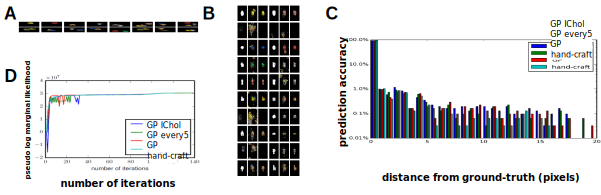
\includegraphics[width=\textwidth]{inveca/invec_mod.pdf}\\
          %  \end{center}
            %
           \begin{itemize}
            \item \highlight{Problem}: locate objects in scene (\textbf{A}), with \textcolor{red}{massive latent space complexity -- $\#$ of obj. locations exponentiated by $\#$ of objects}.
            \item \highlight{Speed}: partial incomplete Cholesky approx to for faster GP regression computation, update GP hyperparams every 5 EM its
            \item \highlight{Shown}: all 3 variants of GP-selection \textcolor{dg}{learn all objects} (\textbf{B}) with \textcolor{dg}{accuracy equivalent to hand-crafted selection} (\textbf{C} \& \textbf{D})
   
          \end{itemize}
\vspace{-.9cm}
    \end{block}




  \end{column} %3

  \end{columns} % all


  %%%%%%%%%%%%%%%%%%%%%%%%%%%%%%%%%%%%%%%%%%%%%%%%%%%%%%%%%%%%%%%%%%%%%%%%%%%
  % References 
  \smallblock{References}{%\& Acknowledgements}{
    \vspace{-.7cm}
    \begin{columns}[t]
      \begin{column}{.52\linewidth}
        \scriptsize
        \lbrack1\rbrack \ Dai, Z. and Lücke, J. (2014). Autonomous document cleaning – a generative approach
to reconstruct strongly corrupted scanned texts. IEEE Transactions on Pattern Analysis and Machine Intelligence (PAMI), 36(10):1950–1962.\

%[3] M.J. Wainwright and M.I. Jordan. Graphical models, exponential families, and variational inference. Foundations and Trends in Machine Learning, 1(1-2), 2008.
%[4] Daphne Koller and Nir Friedman. Probabilistic graphical models: principles and techniques. MIT press, 2009.
%[5] Sameer Singh, Michael L. Wick, and Andrew McCallum. Monte carlo mcmc: Efficient inference by approximate sampling. In EMNLP-CoNLL, pages 1104–1113. ACL, 2012.
        \lbrack2\rbrack \  J. L\"ucke and J. Eggert. (2010). Expectation Truncation And the Benefits of Preselection in Training Generative 
            Models. Journal of Machine Learning Research (JMLR).
        %\lbrack5\rbrack \ \\
        %\lbrack5\rbrack \ \\
        %\lbrack6\rbrack \ \\ 
      \end{column}

    \vspace{-.7cm}
      \begin{column}{.45\linewidth}
        %\small
        %Work supported by the German Research Foundation (DFG) in the project LU~1196/4-1 (JL), 
        %the German Federal Ministry of Education and Research (BMBF), project 01GQ0840 (JAS, JB, ASS), 
        %the Swartz Foundation and the Swiss National Science Foundation (PB),
        %the Physics Dept., and the Center for Scientific Computing (CSC) in Frankfurt.
        %
        %We would like to thank bunnies of the world, and pony's.
        \scriptsize
        \lbrack3\rbrack \ Bornschein, J., Henniges, M., and Lücke, J. (2013). Are V1 simple cells opti-
mized for visual occlusions? A comparative study. PLoS Computational Biology, 9(6):e1003062.\\
        \lbrack4\rbrack \ Sheikh, A.-S., Shelton, J., and Lücke, J. (2014). A truncated EM approach for spike-
and-slab sparse coding. Journal of Machine Learning Research (JMLR), 15:2653–2687.
      \end{column}
    \end{columns}
    }
%
\end{frame}
\end{document}


